\documentclass[tikz,border=5pt]{standalone}
\usepackage{amsmath}
\usetikzlibrary{arrows.meta,positioning,calc}

\definecolor{siteaccent}{RGB}{54,117,138}
\definecolor{sitelight}{RGB}{238,245,247}
\definecolor{siteborder}{RGB}{190,211,218}
\definecolor{sitetext}{RGB}{32,39,43}
\definecolor{sitemuted}{RGB}{102,116,123}

\tikzset{
  block/.style={draw=siteborder, fill=sitelight, rounded corners=2pt,
    minimum width=27mm, minimum height=13mm, align=center, inner xsep=4pt, text=sitetext},
  strong/.style={draw=siteaccent, fill=white, rounded corners=2pt,
    minimum width=29mm, minimum height=13mm, align=center, inner xsep=4pt, text=sitetext},
  flow/.style={-{Latex[length=2.2mm]}, semithick, draw=siteaccent}
}

\begin{document}
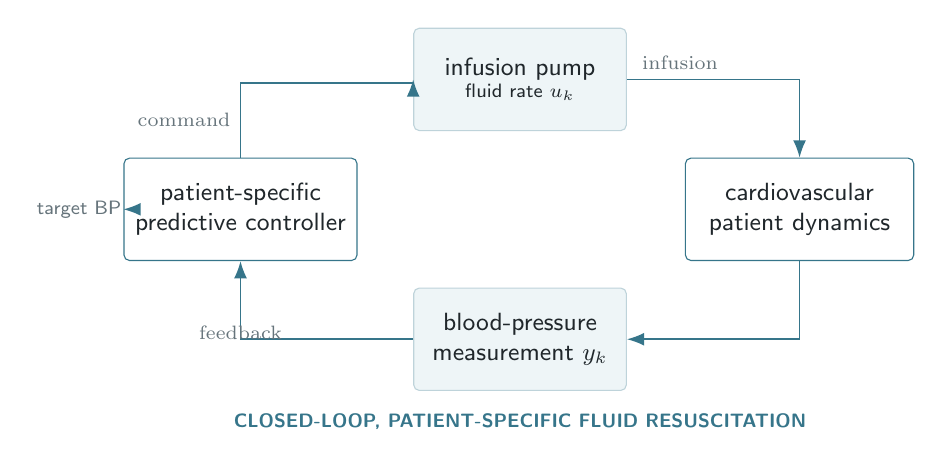
\begin{tikzpicture}[font=\sffamily\small]
  \node[strong] (controller) at (0,0) {patient-specific\\predictive controller};
  \node[block] (pump) at (3.55,1.65) {infusion pump\\[-1mm]\scriptsize fluid rate $u_k$};
  \node[strong] (patient) at (7.1,0) {cardiovascular\\patient dynamics};
  \node[block] (sensor) at (3.55,-1.65) {blood-pressure\\measurement $y_k$};
  \node[text=sitemuted, font=\sffamily\scriptsize] (target) at (-2.05,0) {target BP};

  \draw[flow] (controller.north) -- node[left, text=sitemuted, font=\scriptsize] {command} ++(0,0.95) -| (pump.west);
  \draw[flow] (pump.east) -- node[above, text=sitemuted, font=\scriptsize] {infusion} ++(1.35,0) -| (patient.north);
  \draw[flow] (patient.south) |- (sensor.east);
  \draw[flow] (sensor.west) -| node[pos=0.65, below, text=sitemuted, font=\scriptsize] {feedback} (controller.south);
  \draw[flow] (target) -- (controller.west);

  \node[anchor=north, text=siteaccent, font=\sffamily\scriptsize\bfseries]
    at (3.55,-2.48) {CLOSED-LOOP, PATIENT-SPECIFIC FLUID RESUSCITATION};
\end{tikzpicture}
\end{document}
